\chapter{Results}
\label{chap:results}

The results of four simple benchmarks of WARP against Serpent 2.1.18 and MCNP 6.1 are presented in this section.  All of the benchmarks make use nuclear data loaded from the ACE libraries that Serpent uses.  MCNP 6.1 uses the nuclear data distributed with it, which is also from ENDFB/VII, but since the library files are identical between Serpent and WARP, the error comparisons in this section are made against Serpent, not MCNP.  WARP only uses collision estimators for flux tallies and $k_\mathrm{eff}$ estimations, so the collision estimates from Serpent and MCNP are also used.  Serpent and MCNP have more sophisticated estimators as well, but a comparing WARP against their collision estimators specifically will provide the fairest comparison.  Serpent and MCNP are also run serially, which gives them the best theoretical performance when is comes to scaling, i.e. they are assumed to scale perfectly linearly.  In this way, the card that WARP runs on can be equivocated to a certain number of CPU cores, and a conservative performance per cost comparison can be made.

All of the benchmark cases were run on a server containing two AMD Opteron 6128 Magny-Cours processors.  These processors each contain eight cores which are clocked at 2.0Ghz and have a 512kB L2 cache.  The server has 32 GB of DDR3 clocked at 1.333GHz between the two processors.  The GPU used in the benchmarks is a NVIDIA Tesla k20.  It has 2496 ``CUDA cores,'' a multiprocessor clock of 706MHz, and 5GB of 2.6GHz GDDR5 global memory.  The Opteron 6128 was released in Q2 of 2010, whereas the k20 was released in Q4 2012 \cite{opterondate,k20date}.  This is a comparison of one of the newest Tesla cards with a older CPU, but it is a standard CPU for many supercomputer systems currently running and is sufficient if given every advantage in the comparison (i.e. perfect scaling linearity).

The multiplication factor differences are reported in ``per cent mille,'' which is a thousandth of a percent, or $10^{-5}$.  This is a standard way of reporting differences in the multiplication factor, as any small deviation from unity can cause a reactor to change its power level.  The flux spectra are normalized per source neutron and per lethargy.  Normalizing per source neutron serves to reproduce the same results for different numbers of histories run.  The uncertainty will be lower in results with more histories, of course, but the magnitudes should have the same mean values.   ``Lethargy'' means the logarithm of the neutron energy, $\ln(E_0/E)$, and is convenient since neutrons lose a fraction of energy per collision \cite{duderstadt}.  Normalizing the flux per lethargy accentuates the the high energy region of the flux, and is convenient in plotting spectra since otherwise overshadowed structure in the high-energy regions can be seen.  To plot the raw tally values, shown in \eqref{flux_tally}, the values must be divided by the total number of source neutrons run, divided by the energy bin width to , and multiplied by the average bin energy to normalized by lethargy \cite{lethargyplot}.  The expression for normalizing the raw tally scores is shown in \eqref{fluxtallynorm}, where $\bar{\phi}_{g,j}$ is the raw tally value in cell volume $j$ and energy group $g$.  Since WARP does not include S($\alpha$,$\beta$) or unresolved resonance tables (yet), these features were not activated in MCNP or Serpent in the benchmark runs.  WARP is currently only able to handle black, or vacuum, boundary conditions, so all the benchmark runs use black boundary condition as well.

\begin{equation}
\label{fluxtallynorm}
\begin{gathered}
E_g < E_i < E_{g+1} \\
|\bar{\phi}_{g,j}| = \left( \frac{1}{N_\mathrm{total}}\right) \left(\frac{1}{E_{g+1}-E_g}\right) \left(\frac{E_g+E_{g+1}}{2} \right) \bar{\phi}_{g,j}
\end{gathered}
\end{equation}

Five benchmark cases were considered, four that are criticality-source type, and one that is a fixed-source type.  WARP can represent spheres, cuboids, cylinders, and hexagonal prisms, and all but the hexagonal prism are represented in the benchmarks.  Most of the cases have very simple geometries with few cells, but the assembly case has 632 total cells to accentuate the geometry processing routines and the impact of the material resampling as the neutrons move into different regions without interacting.  Every material in every benchmark case uses some combination of Pu-239, U-238, U-235, O-16, B-10, and H-1.  This is a relatively small set of isotopes to have in a reactor simulation, but loading and processing of isotopes was only tested with Al-27, Pb-208, C-12, Li-6 in addition to these isotopes.  Currently a temperature of 300K is hardcoded into WARP, so cross sections used in these benchmarks are all processed at this temperature.   The summary of the benchmark geometries and materials is shown in Table \ref{benchmark_setup}.  

The ``Jezebel'' benchmark is a bare plutonium sphere, and is a standard criticality test.   The fission neutrons rate from Pu-239 is balanced by the leakage rate from the 5.1cm radius to give a $k_\mathrm{eff}$ of approximately 1.  Since this system is so leaky, producing results consistent with MCNP and Serpent ensure that the boundary conditions are correctly being enforced.  

The ``homogenized block'' benchmark consists of a single cell and a single material as well, but that material has multiple isotopes in it.  This particular material is a one-to-one mixture of 1\% U-235 enriched UO$_2$ and water.  The cell dimensions are quite large as well to emphasize material processing instead of leakage.

The ``pin cell'' benchmark consists of bare UO$_2$ cylinder surrounded by a block of water.  This benchmark now has two materials, each with multiple isotopes, and two cells.  The water block dimensions are not very large, so leakage should play a part.  This benchmark serves to highlight all the processing routines work simultaneously, and the effect of introducing more than one cell, which should have a significant effect on the ray tracing rate as pointed out in the preliminary OptiX study.

The ``15-sided Hex Assembly'' benchmark consists of 631 bare UO$_2$ cylinders laid out in a hexagonal lattice surrounded by water.  The material compositions, densities, and the cylinder dimensions are identical to the pin cell benchmark case, but since this benchmark has two orders of magnitude more objects, it serves to highlight the effect of introducing many geometric objects into the problem and will further validate that the geometry processing routines work correctly if consistent results are obtained.

The ``Fixed-source Block'' benchmark is identical to the homogenized block benchmark in terms of geometry and materials, except for the addition of a small amount B-10 to supress the multiplication factor as to not make runtimes extremely long (the multiplication for $k_\mathrm{eff}$=0.94 is about 17).   A 1eV isotropic point source at the origin was chosen as to highlight the effectiveness of popping any secondary neutrons back into the active transport cycle.  Since the source is at 1eV, it will induce fissions in U-235 which will produce neutrons in a fission spectrum that does not overlap with the source.  

\begin{table}[h]
\centering
\caption{The five benchmark cases.}
\label{benchmark_setup}
\begin{tabular}{| l | c | c | c | c |}
 \hline
 Benchmark & No. Cells & Materials & Isotopes & Densities \\
 \hline
  \hline
 Jezebel                           & 1 sphere, r=5.1cm & Fuel & (1.00) Pu-239 & 19.816 g/cm$^3$\\
  \hline
 \multirow{4}{*}{Homogenized Block}  & \multirow{4}{*}{1 cube, 2m$^3$ } & \multirow{4}{*}{Hom. Fuel.} & (0.99) U-238  & \multirow{4}{*}{10  g/cm$^3$} \\
 & & & (0.01) U-235 & \\
 & & & (3.00) O-16   & \\
 & & & (2.00) H-1     & \\
  \hline
 \multirow{5}{*}{Pin Cell}                        & \multirow{4}{*}{1 cuboid, 10x10x50cm} & \multirow{3}{*}{Fuel} & (0.90) U-238 & \multirow{3}{*}{15  g/cm$^3$} \\
 &  \multirow{4}{*}{1 cylinder, r=1cm z=40cm} & & (0.10) U-235 & \\
  & & & (2.00) O-16 & \\
 \cline{3-5}
 & & \multirow{2}{*}{Water} & (1.00) O-16 &  \multirow{2}{*}{3  g/cm$^3$} \\
 & & & (2.00) H-1 & \\
  \hline
  \multirow{4}{*}{15-sided}  & \multirow{4}{*}{1 cube, 84cm$^3$} & \multirow{3}{*}{Fuel} & (0.90) U-238 & \multirow{3}{*}{15  g/cm$^3$} \\
 \multirow{4}{*}{Hex Assembly}   & \multirow{4}{*}{631 cylinders, r=1cm z=40cm} & & (0.10) U-235 & \\
     & & & (2.00) O-16 & \\
 \cline{3-5}
 & & \multirow{2}{*}{Water} & (1.00) O-16 &  \multirow{2}{*}{3  g/cm$^3$} \\
 & & & (2.00) H-1 & \\
  \hline
 \multirow{5}{*}{Fixed-source Block}  & \multirow{4}{*}{1 cube, 2m$^3$ } & \multirow{4}{*}{Hom. Fuel.} & (0.99) U-238  & \multirow{4}{*}{10  g/cm$^3$} \\
 & &  \multirow{4}{*}{with B-10} & (0.01) U-235 & \\
 & & & (3.00) O-16   & \\
 & & & (0.01) B-10   & \\
 & & & (2.00) H-1     & \\  
 \hline
 \end{tabular}
\end{table}

%%%%%%%%%%%%%%%%%%%%%%%%%%%%%%%%%%%%%%%%%%%%%%
%%%%%%%%%%%%%%%%%%%%%%%%%%%%%%%%%%%%%%%%%%%%%%
\section{Multiplication Factors and Runtimes}

The goal of WARP is to be the first step in creating a full-featured continuous energy Monte Carlo neutron transport code that is \emph{accelerated} by running on GPUs.  The crux of the effort is to make Monte Carlo calculations faster but still produce accurate results.  Table \ref{benchmark_summary_5} shows the multiplication factor deviations and the speedup factors for the four criticality benchmarks compared to MCNP 6.1 and Serpent 2.1.18 when $10^5$ neutrons per batch are used.  Table  \ref{benchmark_summary_6} shows the same information, but for cases where $10^6$ neutrons per batch are used.

\begin{table}[h]
\centering
\caption{Summary of $k_\mathrm{eff}$ single-run results of the WARP criticality benchmarks with 20/40 discarded/active criticality cycles and $10^5$ histories per cycle.}
\label{benchmark_summary_5}
\begin{tabular}{| l | r | r | r | r | r |}
 \hline
 Benchmark & MCNP 6.1 & Serpent 2.1.18 & WARP & $\Delta$ M & $\Delta$ S  \\
\hline
\hline
\multicolumn{6}{|l|}{Jezebel}  \\
\hline
 $k_\mathrm{eff}$ & 1.027509$\pm$0.0005 & 1.02748$\pm$0.00052 & 1.02789 & -38.1 pcm (y) & -41 pcm (y) \\
 \hline
 Runtime               & 2.32 m & 9.50868 m & 0.2752 m & 8.4x  & 34.6x  \\
 \hline
 \hline
\multicolumn{6}{|l|}{Homogenized Block }\\
\hline
 $k_\mathrm{eff}$ & 0.943049$\pm$0.0003 & 0.940306$\pm$0.00046 & 0.941916 & 113 pcm (n)  & -161 pcm  (n) \\
 \hline
 Runtime               &  25.58 m & 18.7190 m & 0.761 m & 33.6x  & 24.6x  \\
 \hline
  \hline
\multicolumn{6}{|l|}{Pin Cell}\\
\hline
 $k_\mathrm{eff}$ & 0.381435$\pm$0.0008 &  0.380511$\pm$0.00128 & 0.380586 & 84.9 pcm (n)&  -7.5 pcm (y)    \\
 \hline
 Runtime               & 55.85 m & 40.0035 m &  2.81583 m &  19.8x & 14.2x  \\
 \hline
  \hline
\multicolumn{6}{|l|}{15-sided Hex Assembly}\\
\hline
 $k_\mathrm{eff}$ & 1.437465$\pm$0.0004 & 1.44704$\pm$0.00046 & 1.4442 & -673 pcm (n) & 284 pcm (n) \\
 \hline
 Runtime               & 25.34 m &  26.3349 m &  3.2395 m  & 7.8x & 8.1x  \\
 \hline
\end{tabular}
\end{table}


\begin{table}[h]
\centering
\caption{Summary of $k_\mathrm{eff}$ single-run results of the WARP criticality benchmarks with 20/40 discarded/active criticality cycles and $10^6$ histories per cycle.}
\label{benchmark_summary_6}
\begin{tabular}{| l | r | r | r | r | r |}
 \hline
 Benchmark & MCNP 6.1 & Serpent 2.1.18 & WARP & $\Delta$ M & $\Delta$ S  \\
\hline
\hline
\multicolumn{6}{|l|}{Jezebel}  \\
\hline
 $k_\mathrm{eff}$ & 1.027957$\pm$0.0001 & 1.02806$\pm$0.00017 & 1.0279 & 5.7 pcm (y)& 16 pcm  (y) \\
 \hline
 Runtime               & 22.79 m & 94.4311 m &  2.0147 m & 11.3x  & 46.9x  \\
 \hline
 \hline
\multicolumn{6}{|l|}{Homogenized Block }\\
\hline
 $k_\mathrm{eff}$ & 0.942670$\pm$0.0001 & 0.939868$\pm$0.00021 & 0.94261 & 6 pcm (y) &  -274.4 pcm (n)  \\
 \hline
 Runtime               & 255.57 m & 185.966 m & 3.934 m & 64.96x & 47.28x  \\
 \hline
  \hline
\multicolumn{6}{|l|}{Pin Cell}\\
\hline
 $k_\mathrm{eff}$ & 0.381405$\pm$0.0003 & 0.380615$\pm$0.00035 & 0.38043 & 97.5 pcm (n) &  18.5 pcm (n)  \\
 \hline
 Runtime               & 578.62 m & 391.995 m & 7.0682 m & 81.85x & 55.46x \\
 \hline
  \hline
\multicolumn{6}{|l|}{15-sided Hex Assembly}\\
\hline
 $k_\mathrm{eff}$ & 1.437711$\pm$0.0001 & 1.44706$\pm$0.00013 & 1.4454 & -769 pcm (n) &  166 pcm (n) \\
 \hline
 Runtime               & 252.77 m & 260.508 m & 7.9703 m & 31.71x & 32.68x \\
 \hline
\end{tabular}
\end{table}

It can be seen that in the $10^5$ neutrons per batch case, WARP performs 8 to 35 times faster than the production codes, and the multiplication factor differences are slightly different.  Most multiplication factors are most notably different in the assembly benchmark, where WARP's answer falls between MCNP and Serpent, but is still very far from either.  Similar trends are shown in the multiplication factor for the $10^6$ runs in Table \ref{benchmark_summary_6}, but the speedup factors are much higher, with WARP being 11 to 82 times faster than the production codes.   The greatest speedup is seen in the pin cell benchmark, followed by the homogenized block, assembly, then finally the bare sphere.  The speedup factors compared to Serpent in the $10^6$ neutrons per batch runs are relatively constant, ranging from 33 to 56, whereas the speedup factors compared to MCNP range from 11 to 82.

The (y) in the $\Delta$ columns signify if the WARP value is inside (y) or outside (n) one standard deviation of the production code's value.  In the Jezebel benchmark, all codes agree, but as things get more complicated, deviations start to occur.  WARP is often outside of a single standard deviation for either code.  It is important to point out that Serpent and MCNP are also often more than a standard deviation away from each other, with WARP falling somewhere in between, or if not in between, near one of the two codes.

It is also interesting that in the Jezebel benchmark, MCNP is actually much faster than Serpent.  Presumably, this is do to the different methods they use for neutron tracking.  Serpent uses Woodcock tracking, and moves the neutron in small steps across the geometry, but does not have to calculate any surface intersection points.  MCNP uses ray tracing and does calculate intersection points (as does WARP).  Since the Jezebel sphere is a very leaky system, many neutrons stream out of the sphere without interacting many times or at all.  Since  MCNP and WARP both use ray tracing, they can terminate this particles in a small number of geometry queries.  Serpent, however, needs to query the geometry many times in order to propagate the neutrons to the edge of the sphere where they are then leaked.  This difference is not seen in the homogenized block benchmark, where leakage plays very little role in neutron loss.

%%%%%%%%%%%%%%%%%%%%%%%%%%%%%%%%%%%%%%%%%%%%%%
%%%%%%%%%%%%%%%%%%%%%%%%%%%%%%%%%%%%%%%%%%%%%%
\section{Flux Spectra and Fission Distributions}

\begin{figure}[h!] 
\centering
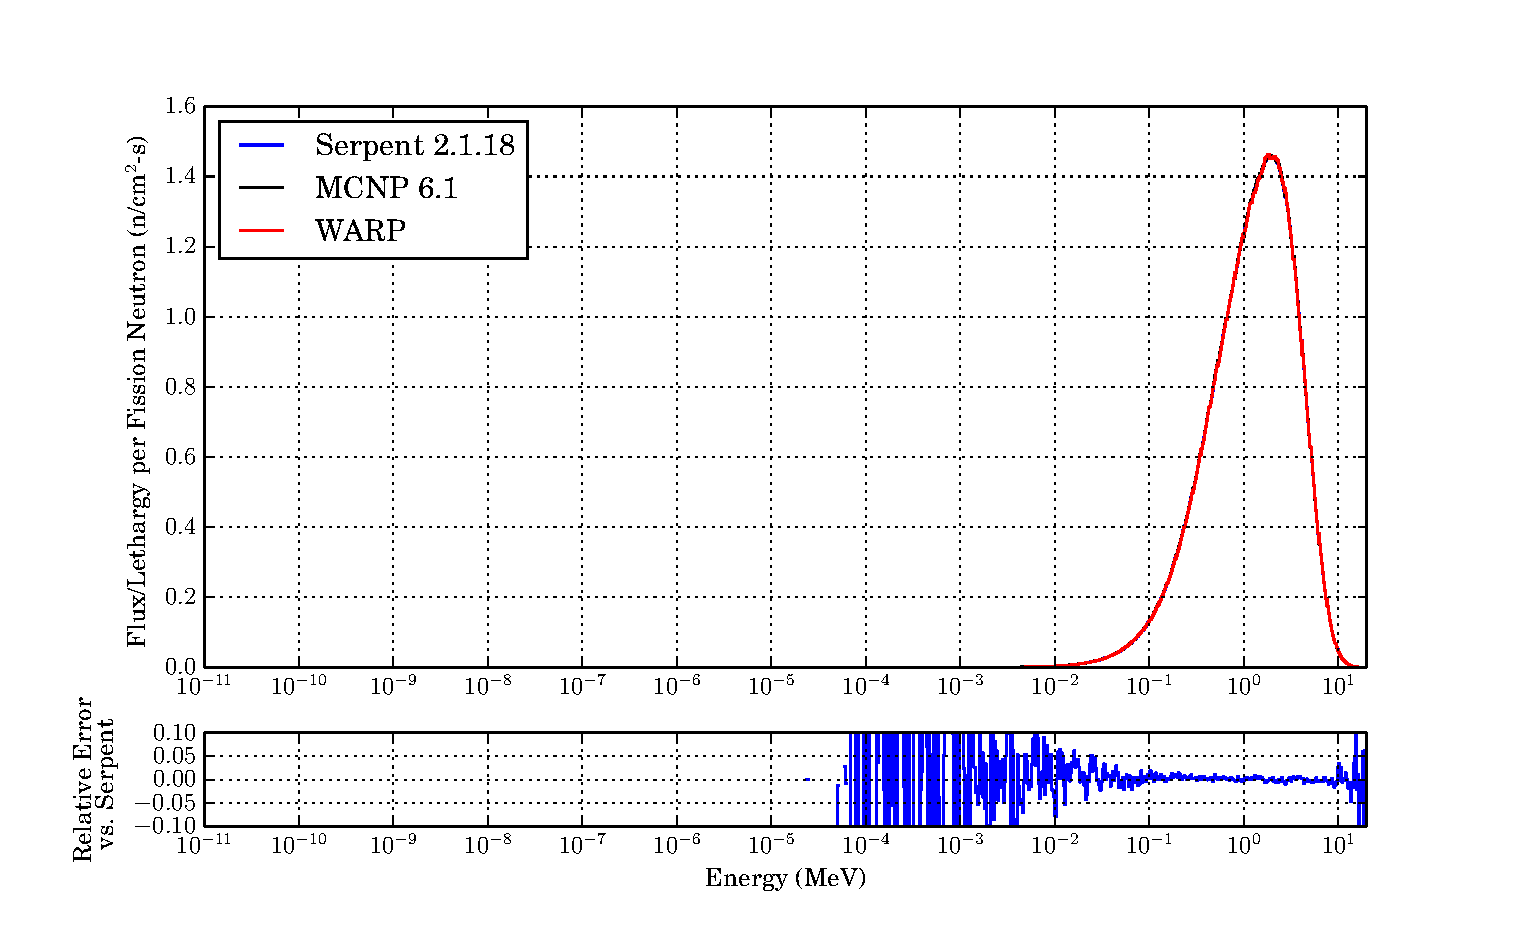
\includegraphics[width=\textwidth,trim= 1cm 0cm 1cm 0cm]{graphics/finalresults/godiva_spec-6.eps}
\caption{Spectrum comparison in a ``Jezebel'' bare Pu-239 sphere. \label{godiva_spec} }
\end{figure}

\begin{figure}[h!]
\centering
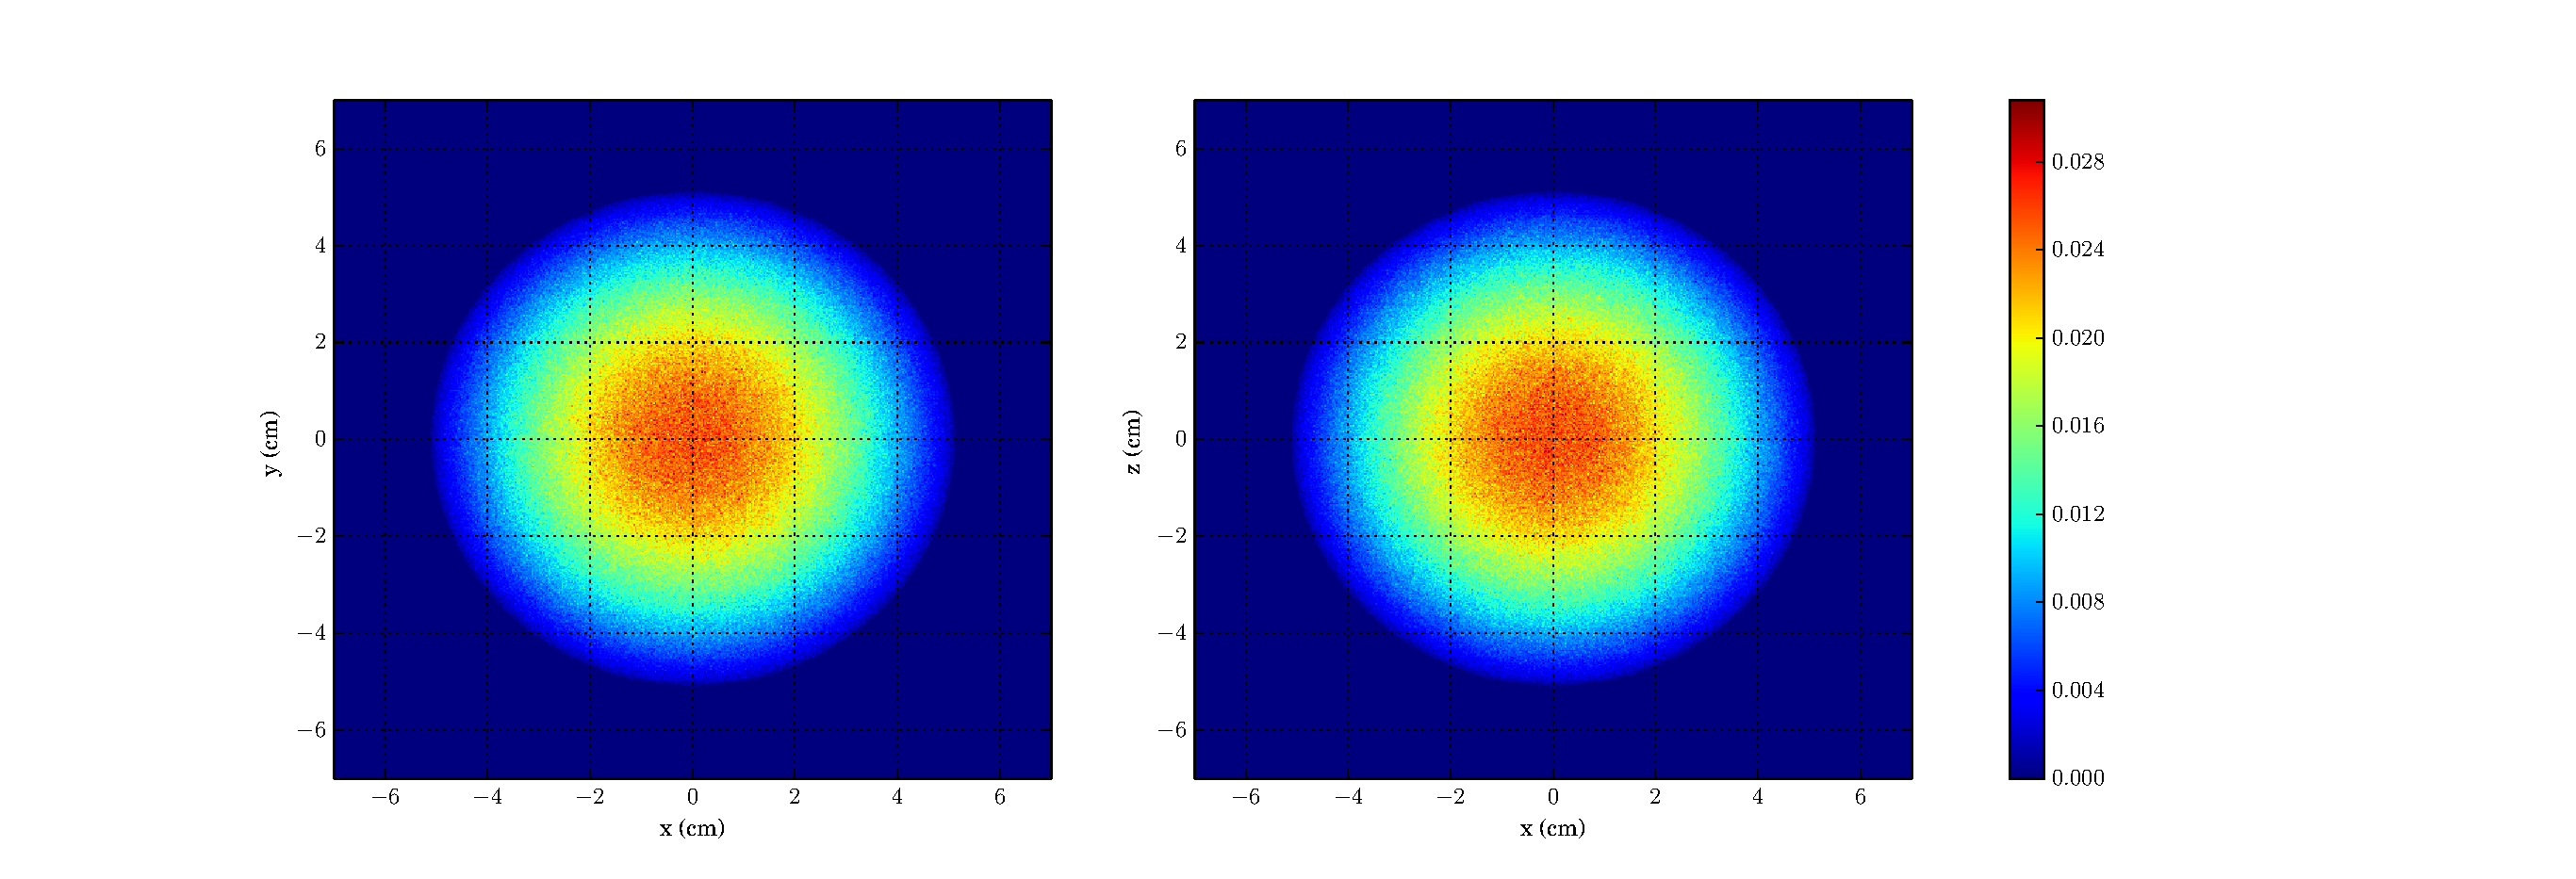
\includegraphics[width=\textwidth,trim= 5cm 0cm 7cm 0cm]{graphics/finalresults/godiva_fiss-6.eps}
\caption{Fission source distribution of a ``Jezebel'' bare Pu-239 sphere. \label{godiva_fiss} }
\end{figure}

\begin{figure}[h!] 
\centering
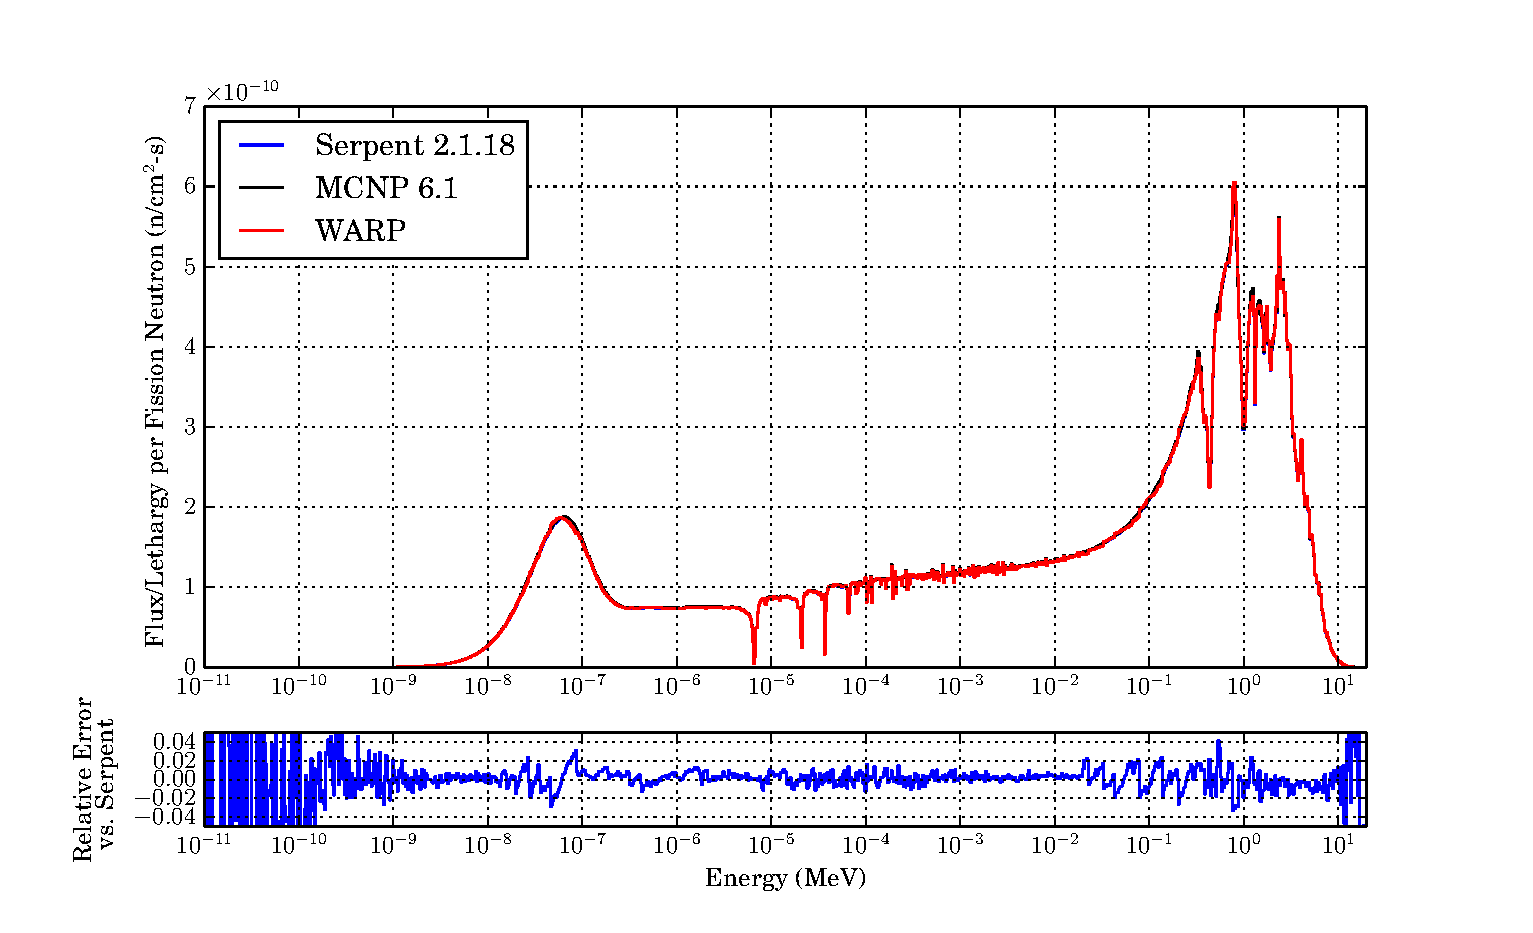
\includegraphics[width=\textwidth,trim= 1cm 0cm 1cm 0cm]{graphics/finalresults/homfuel_spec-6.eps}
\caption{Spectrum comparison in a homogenized block of UO$_2$ and water. \label{homfuel_spec} }
\end{figure}

\begin{figure}[h!]
\centering
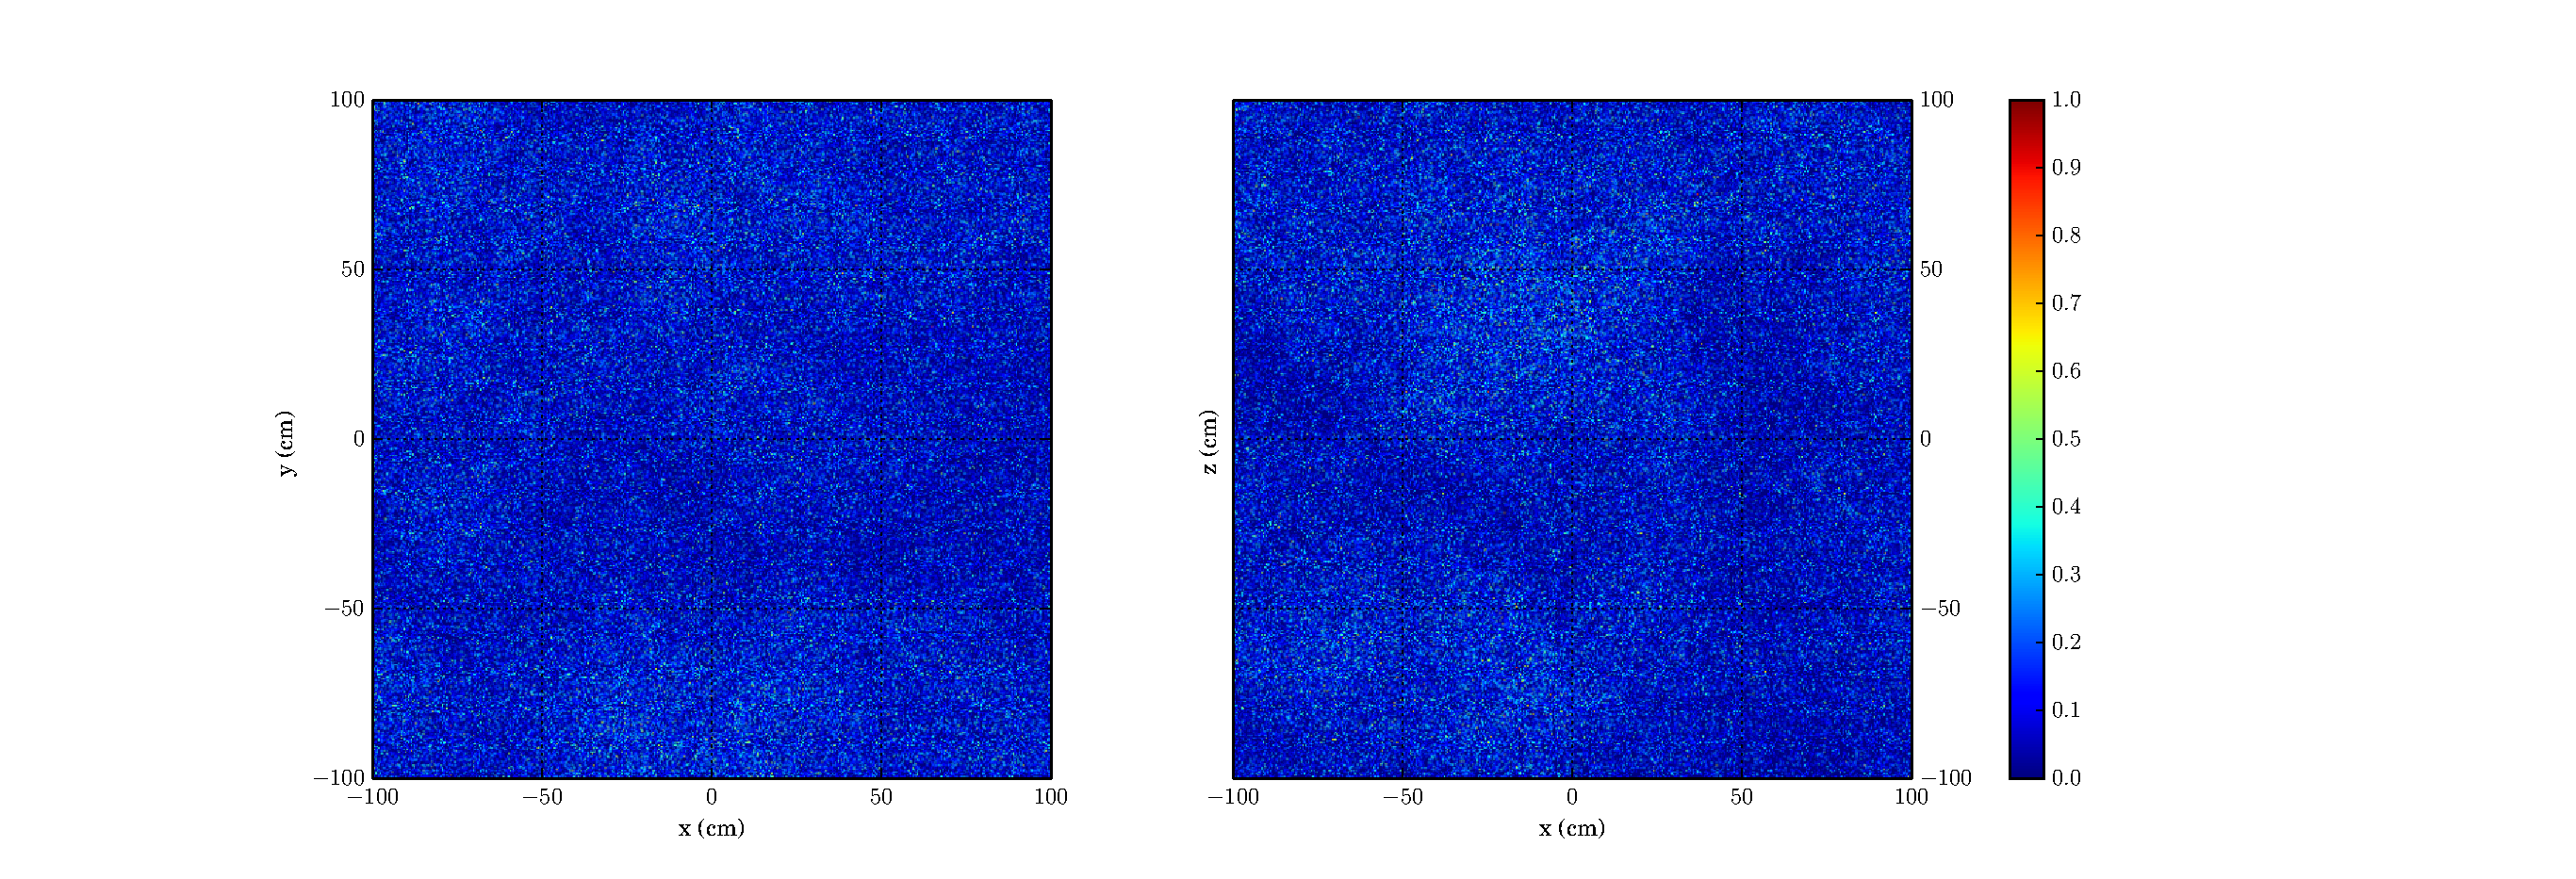
\includegraphics[width=\textwidth,trim= 5cm 0cm 7cm 0cm]{graphics/finalresults/homfuel_fiss-6.eps}
\caption{Fission source distribution of a homogenized block of UO$_2$ and water. \label{homfuel_fiss} }
\end{figure}

The flux and fission source distributions for the criticality benchmarks are shown in the following figures.  The colors in the fission source distribution plots represent the probability density of a fission neutron being born at that point.  To show the most accurate and highest resolution results, the data in these figures are from runs using $10^6$ neutrons per batch.  The corresponding Serpent fission source and thermal flux mesh plots are included in Figures \ref{serp_godiva_mesh}-\ref{serp_assembly_mesh} in Appendix \ref{app:A} so the fission source distributions shown here can be visually validated against them.  

Figures \ref{godiva_spec} and \ref{godiva_fiss}, show the volume-averaged flux spectrum and fission source distribution, respectively, in the Jezebel sphere.  The relative error compared to the Serpent spectrum is show in the subplot below the main spectrum plot.  The relative error is very low compared to Serpent, with the normalized tally bins being less than 2\% from each other in regions where the flux is large.  Of course, when the flux is small, the statistical uncertainty becomes much higher, and the relative error becomes noisy.  The spectra produced by the three codes lie very close together and are almost indistinguishable from each other in the plot.  The fission distribution appears very uniform with neutrons being preferentially born near the center.  The distribution is visually identical in an $z$-integrated slice compared to the $y$-integrated slice, as it should be.

Figures \ref{homfuel_spec} and \ref{homfuel_fiss}, show the volume-averaged flux spectrum and fission source distribution, respectively, in the block of homogenized fuel.  Since this system is not leaky and contains light nuclides, neutrons should be able to easily scatter down to thermal energies and produce a thermal peak around 0.026 eV.  This feature is seen in the WARP spectrum, indicating that the target velocity sampling scheme is working correctly, as well as the vector transformation and rotation schemes.  Again, the relative error compared the the Serpent spectrum is very low, at 3\% or lower for energies $10^{-9}$-$10$ MeV where the flux has good statistics.  There are some strange sawtooth-like structures in the relative error plot in the thermal peak and the unresolved resonance regions, which could indicate that a minor sampling problem is occurring, and should be investigated as WARP continues to develop.  The fission source distribution shows very interesting nebulous structure, which might indicate that the fission source has not been fully sampled.  This may be to the fact that the block is so large, but the results should be almost same as a fully converged source since most neutrons never encounter geometry anyway.  The edges falloff to zero as they should, and the overall appearance of the distribution is quite uniform.

Figures \ref{pincell_spec} and \ref{pincell_fiss}, show the volume-averaged flux spectrum and fission source distribution, respectively, in the UO$_2$ pin of the pin cell benchmark.  This system is slightly leaky, and again contains light nuclides (water), but now they are spatially separated from the fissile material.  The relative error compared to Serpent is again low, around 3\% or lower for energies $5\times10^{-9}$-$10$ MeV where the flux has good statistics.  There is a small thermal peak in the spectrum compared to that of the homogenized fuel material.  This is expected behavior as the fuel has a much higher cross section at these energies than the homogenized fuel material.  This effect can also be seen in the fission source distribution as a ring of high probability around the edge of the pin.  This is cause by thermalized neutrons re-entering the fuel pin and immediately fissioning a U-235 nucleus.  This phenomenon is also called ``self-shielding'' since the uranium at the surface shields the interior uranium from thermal neutrons and has implications in depletion and power distributions.  Since the flux spectrum is volume averaged over the pin, the small thermal peak is most likely from the inclusion of this thin edge region where thermal neutrons still exist.  The axial fission source distribution follows an expected behavior of a finite cylinder as well, roughly following a cosine with the peak at $z=0$ \cite{duderstadt}.

 
\begin{figure}[h!] 
\centering
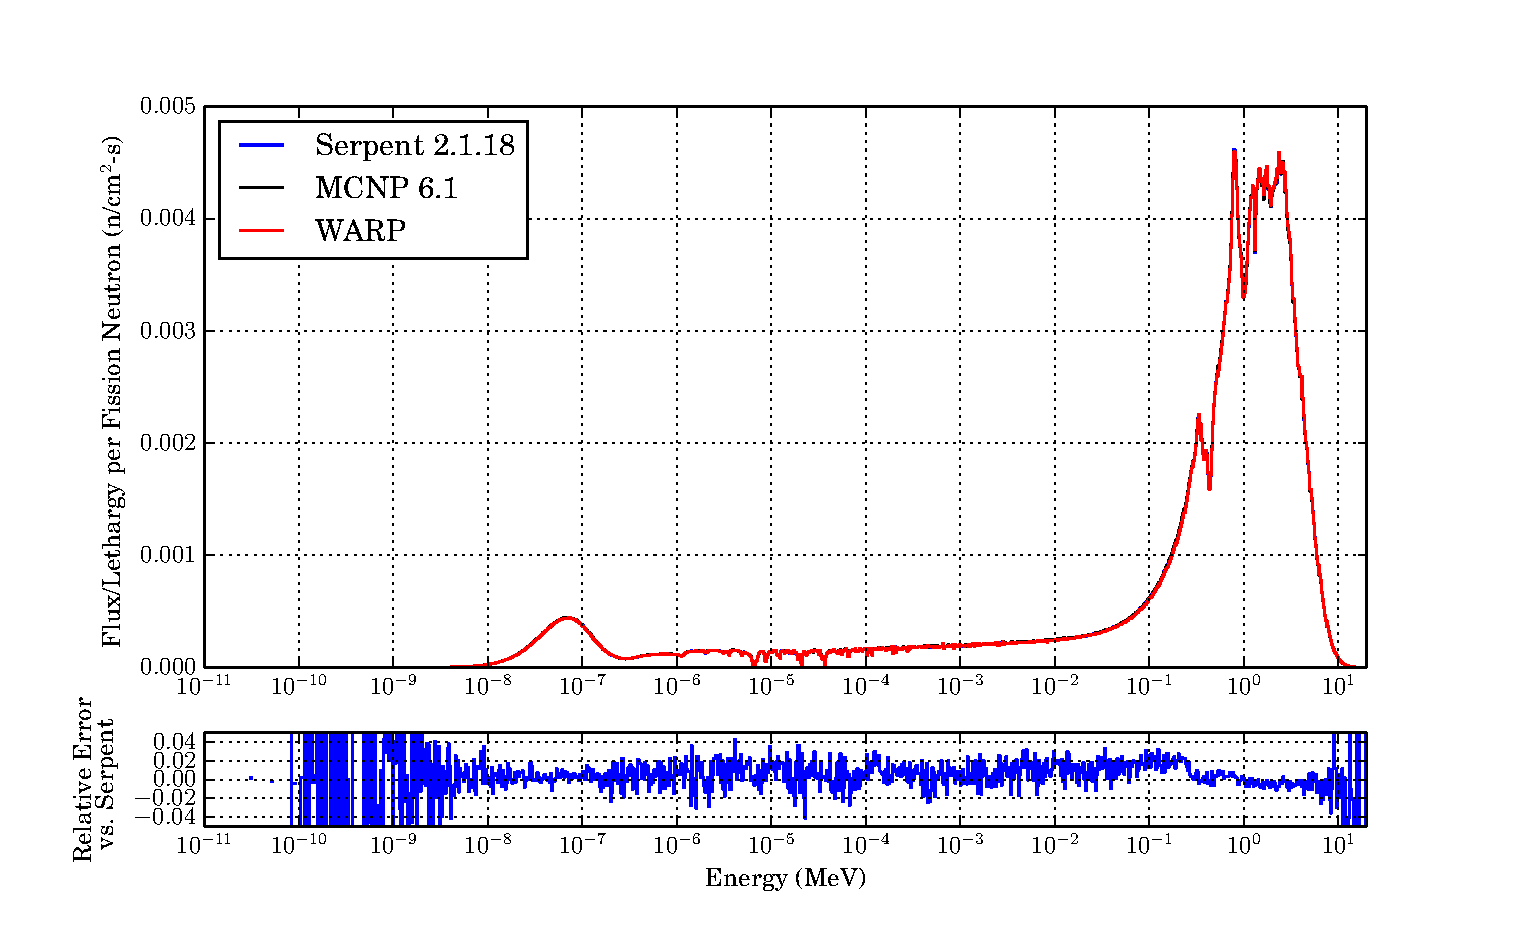
\includegraphics[width=\textwidth,trim= 1cm 0cm 1cm 0cm]{graphics/finalresults/pincell_spec-6.eps}
\caption{Spectrum comparison in a single UO$_2$ pin surrounded by a block of water. \label{pincell_spec} }
\end{figure}

\begin{figure}[h!]
\centering
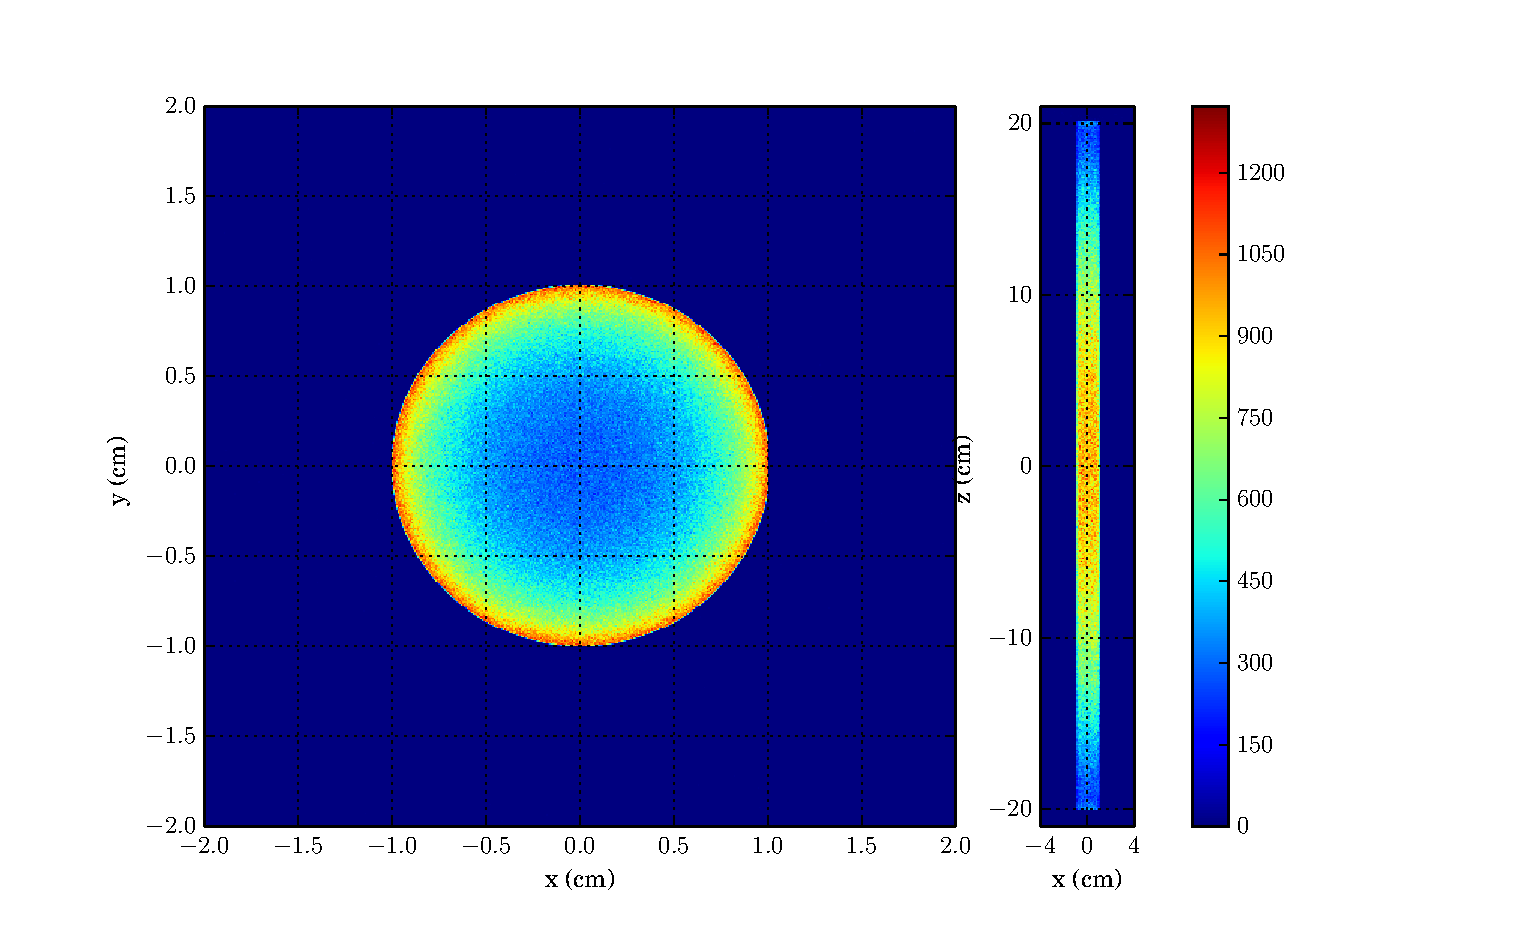
\includegraphics[width=.75\textwidth]{graphics/finalresults/pincell_fiss-6.eps}
\caption{Fission source distribution of a single UO$_2$ pin surrounded by a block of water. \label{pincell_fiss} }
\end{figure}

\begin{figure}[h!] 
\centering
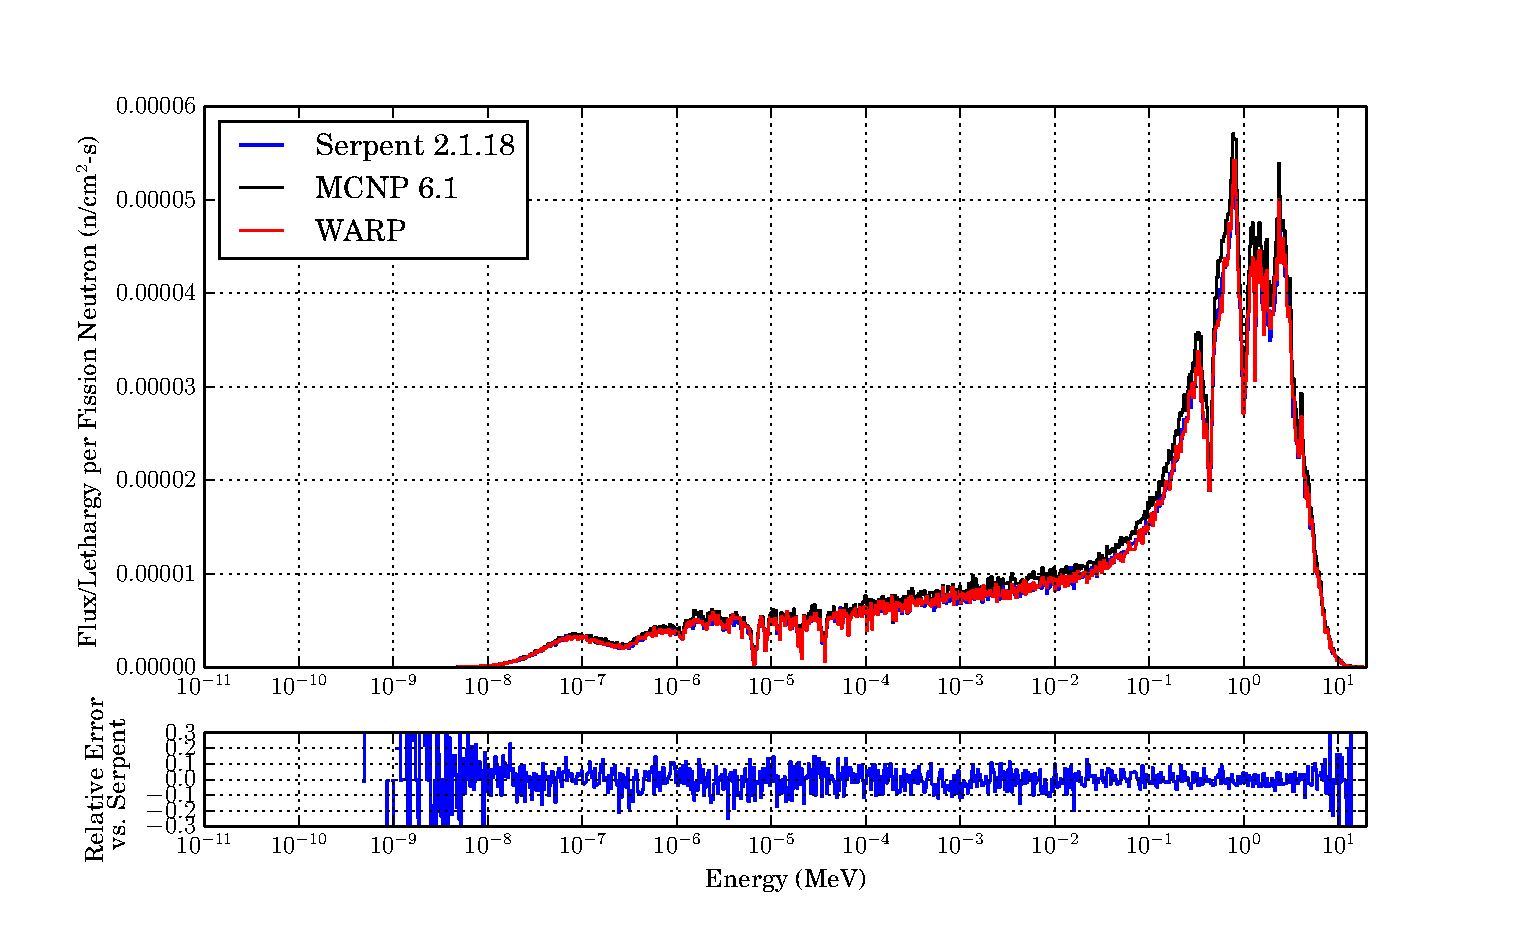
\includegraphics[width=\textwidth,trim= 1cm 0cm 1cm 0cm]{graphics/finalresults/assembly_spec-6.eps}
\caption{Spectrum comparison in the center UO$_2$ pin of a 15-sided hexagonal pin array in water. \label{assembly_spec} }
\end{figure}

\begin{figure}[h!]
\centering
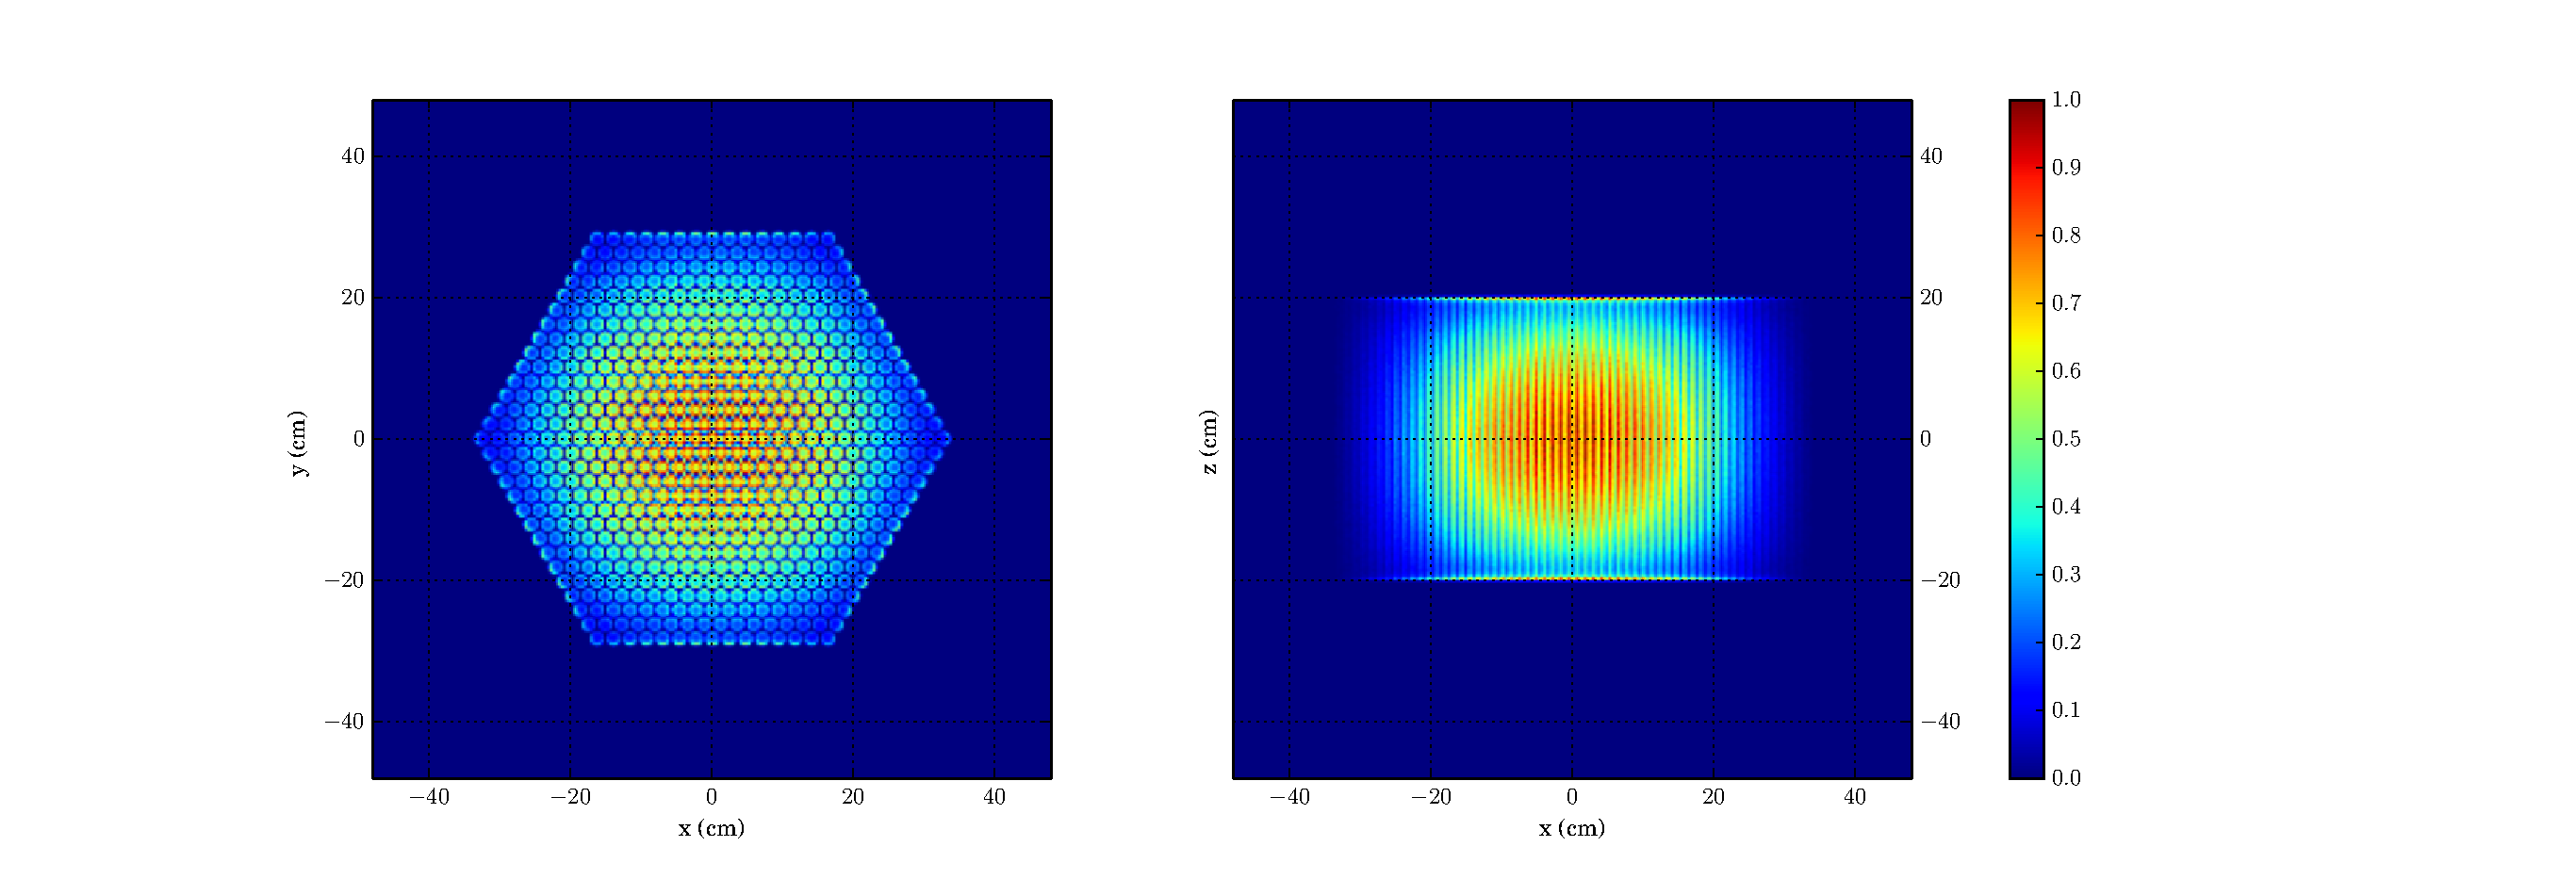
\includegraphics[width=\textwidth,trim= 4cm 0cm 6cm 0cm]{graphics/finalresults/assembly_fiss-6.eps}
\caption{Fission source distribution of a 15-sided hexagonal array of UO$_2$ pins in water. \label{assembly_fiss} }
\end{figure}
	

Figures \ref{assembly_spec} and \ref{assembly_fiss}, show the volume-averaged flux spectrum and fission source distribution, respectively, in the center pin of the 15-sided hexagonal assembly benchmark.  This problem is much more heterogeneous than any of the previous, with 300 times more objects in the domain compared to the pin cell benchmark.  The WARP's spectrum matches very well with Serpent's, and the relative error is with 15\% of Serpent  for energies $10^{-8}$-$9$ MeV where the flux has good statistics.  The spectrum is much noisier than any of the other benchmarks since the volume of the center pin is relatively small compared to the volume of the fission source, even though this pin has the highest flux of any of the pins.  The mean of the error appears to be close to zero, however, and the high error is most likely due to statistics.  The MCNP spectrum is slightly higher than both the WARP and Serpent spectra, which might be a small normalization error or a real difference.  The fission source distribution appears as expected, with the highest average probability in the center of the array both axially and radially.  Self-shielding is shown again, as every pin has a ring of higher probability on near its surface.  The assembly also shows some reflection effects from the thick layers of water surrounding it.  The pins at the edges have a higher fission source probability at the surfaces facing the water rather than the interior of the assembly.  This is due to neutrons being abel to scatter many times in the large volume of water and eventually scattering into an edge pin where there are immediately absorbed.  This phenomenon is apparent in both the axial and radial directions.


%%%%%%%%%%%%%%%%%%%%%%%%%%%%%%%%%%%%%%%%%%%%%%
%%%%%%%%%%%%%%%%%%%%%%%%%%%%%%%%%%%%%%%%%%%%%%
\section{Fixed Source}

WARP is also able to run simulations in fixed-source mode, where the initial neutron energies, directions, and locations are predefined and do not incorporate any feedback from the flux like the criticality source.  This mode adds any induced secondary neutrons back into the active particle dataset to be transported in conjunction with the source neutrons, which is also why these problems must be subcritical.  The materials and geometry are the same as the homogenized block, but with a small amount of B-10 added to reduce the multiplication factor to ensure reasonable runtimes.

\begin{table}[h]
\centering
\caption{Summary of $k_\mathrm{eff}$ single-run results of the WARP fixed-source benchmark with $4^7$ total histories.}
\label{fixed_summary}
\begin{tabular}{| l | r | r | r | r | r |}
 \hline
 & MCNP 6.1 & Serpent 2.1.18 & WARP & $\Delta$ M & $\Delta$ S  \\
\hline
\hline
 $k_\mathrm{eff}$ & 0.18314 (inferred) & 0.270545$\pm$0.00015 & 0.273947 & -9080.7 pcm & -340.2 pcm   \\
 \hline
 Runtime               & 82.32 m & 7.11 m &  3.52 m & 23.4x  & 2.0x  \\
 \hline
\end{tabular}
\end{table}

\begin{figure}[h!]
\centering
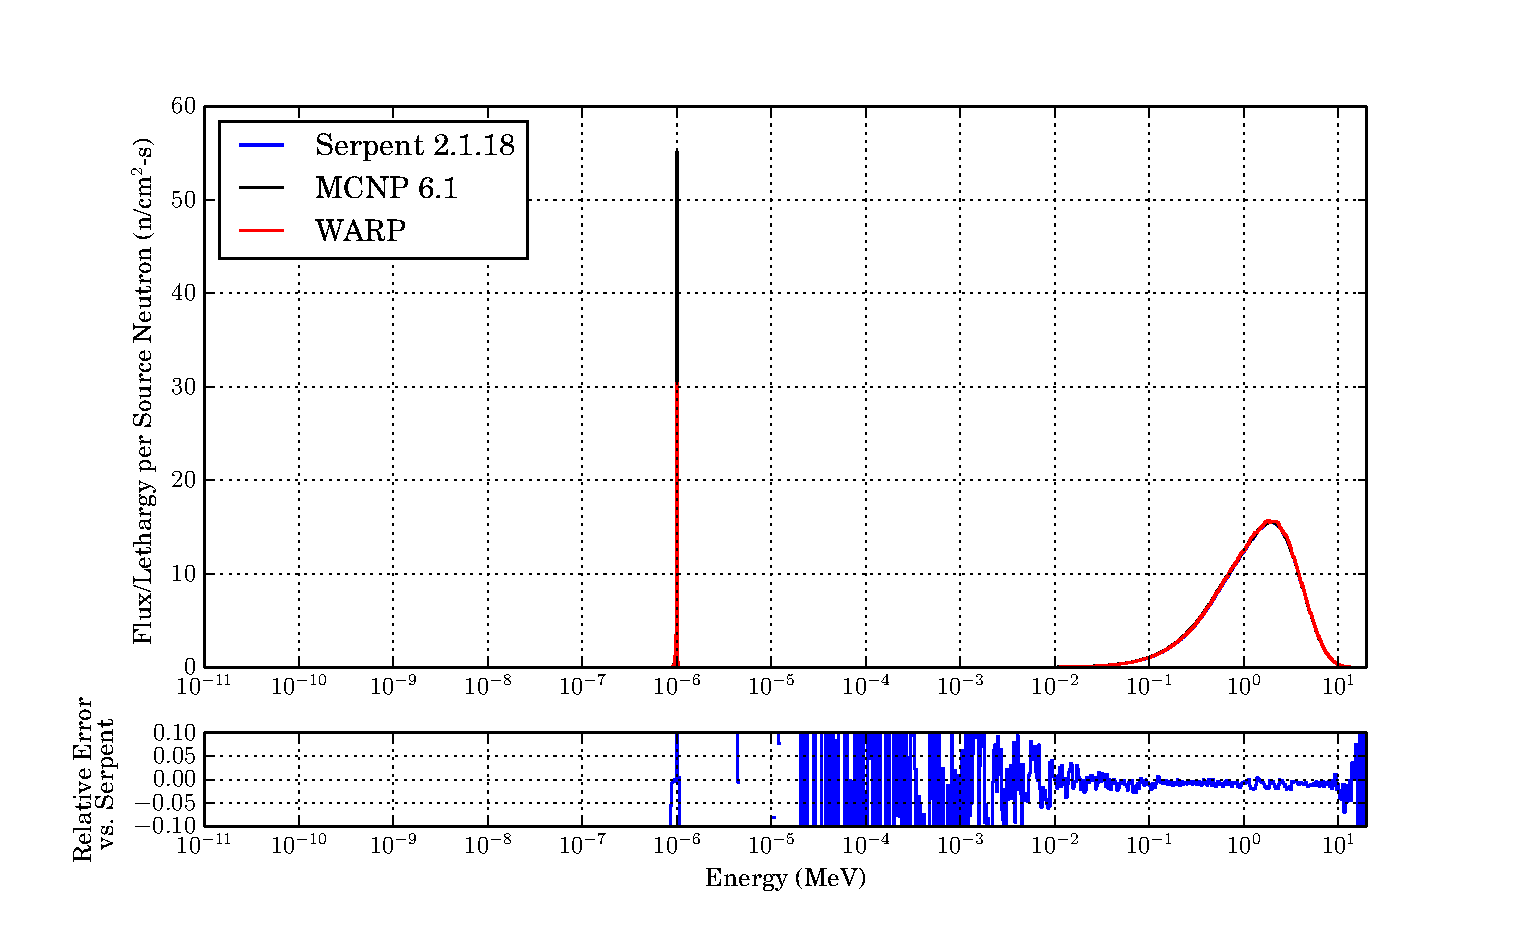
\includegraphics[width=\textwidth,trim= 1cm 0cm 1cm 0cm]{graphics/finalresults/fixed_spec.eps}
\caption{Flux spectra of fixed source calculations of a 1eV points source in a block of uranium-235 . \label{fixed_spec} }
\end{figure}

Table \ref{fixed_summary} shows the runtimes and multiplication factors calculated by WARPM compared to the production codes.  MCNP does not report a multiplication factor when run with a fixed source, so the value shown was inferred via \eqref{sub_crit_mult} using the ``total multiplication'' value that was reported in the MCNP output file.  The value calculated by WARP is near Serpent's, but it is outside one standard deviation.  The inferred value from MCNP is very far from either, and may not be an accurate result.  WARP is moderately faster than Serpent, but substantially faster than MCNP.  Compared to the homogenized block criticality benchmark, the speedup factor compared to Serpent is much lower.  This may be do to the fact that secondary particles are popped into active data after every iteration of the inner transport loop, whereas the source pop only happens at the end of the outer loop in criticality mode.

Figure \ref{fixed_spec} shows a comparison of the spectra produced by WARP compared to Serpent 2.1.18 and MCNP 6.1.  The relative error of the spectrum compared to Serpent is below 2\% for energies $10^{-9}$-$9$ MeV where the flux has good statistics.  The exception to this is at 1 eV, the neutron source energy.  The flux reported by MCNP and Serpent is about twice as high as that reported by WARP at this one point.  The are a few sawtooth structures in the relative error as well, especially in the thermal region below the source energy.  The magnitude of the flux is very small since the volume is large and most neutrons will not travel further than a few centimeters from the source point in this material.

%%%%%%%%%%%%%%%%%%%%%%%%%%%%%%%%%%%%%%%%%%%%%%
%%%%%%%%%%%%%%%%%%%%%%%%%%%%%%%%%%%%%%%%%%%%%%
\section{Comparison to Non-Remapping}

To measure the benefit of sorting and remapping references in WARP, a comparison to a non-remapping version of WARP must be made.  Table \ref{benchmark_nonremapping_summary} shows the runtimes and multiplications factors of the criticality benchmarks for remapping and non-remapping versions of WARP.  The remapping version performs much better than the non-remapping version when more complexity is added to the problem.  For very simple problems, like the Jezebel benchmark, remapping only adds overhead since the neutrons are constrained be the problem materials on geometry to generally do undergo the same three reactions: fission and scattering in Pu-239 or leaking out.  The leaky nature of the problem also means neutrons only undergo a few interactions on average before being terminated.  In the non-remapping case, this is advantageous since the version is less efficient at processing neutrons when the active number is small.

\begin{table}[h]
\centering
\caption{Comparison of the non-remapping and remapping versions of WARP for the four criticality benchmark cases.  20/40 discarded/active criticality cycles and $10^6$ histories per cycle.}
\label{benchmark_nonremapping_summary}
\begin{tabular}{| l | r | r | r |}
 \hline
 Benchmark & Remapping WARP & Non-Remapping WARP & $\Delta k$ or Ratio  \\
\hline
\hline
\multicolumn{4}{|l|}{Jezebel}  \\
\hline
 $k_\mathrm{eff}$ & 1.0279 & 1.0279  & 0 pcm\\
 \hline
 Runtime               &   2.0147 m & 1.84 m & 0.91x \\
 \hline
 \hline
\multicolumn{4}{|l|}{Homogenized Block }\\
\hline
 $k_\mathrm{eff}$ & 0.9426 & 0.941857 & 74.3 pcm  \\
 \hline
 Runtime               &  3.934 m & 4.05 m & 1.03x \\
 \hline
  \hline
\multicolumn{4}{|l|}{Pin Cell}\\
\hline
 $k_\mathrm{eff}$ &  0.3804 & 0.38063  & -23 pcm \\
 \hline
 Runtime               & 7.0682 m & 10.52 m & 1.49x \\
 \hline
  \hline
\multicolumn{4}{|l|}{15-sided Hex Assembly}\\
\hline
 $k_\mathrm{eff}$  & 1.4454  & 1.4457 & -30 pcm \\
 \hline
 Runtime               & 7.9703 m & 95.85 m & 12.03x \\
 \hline
\end{tabular}
\end{table}

\begin{figure}[h!]
\centering
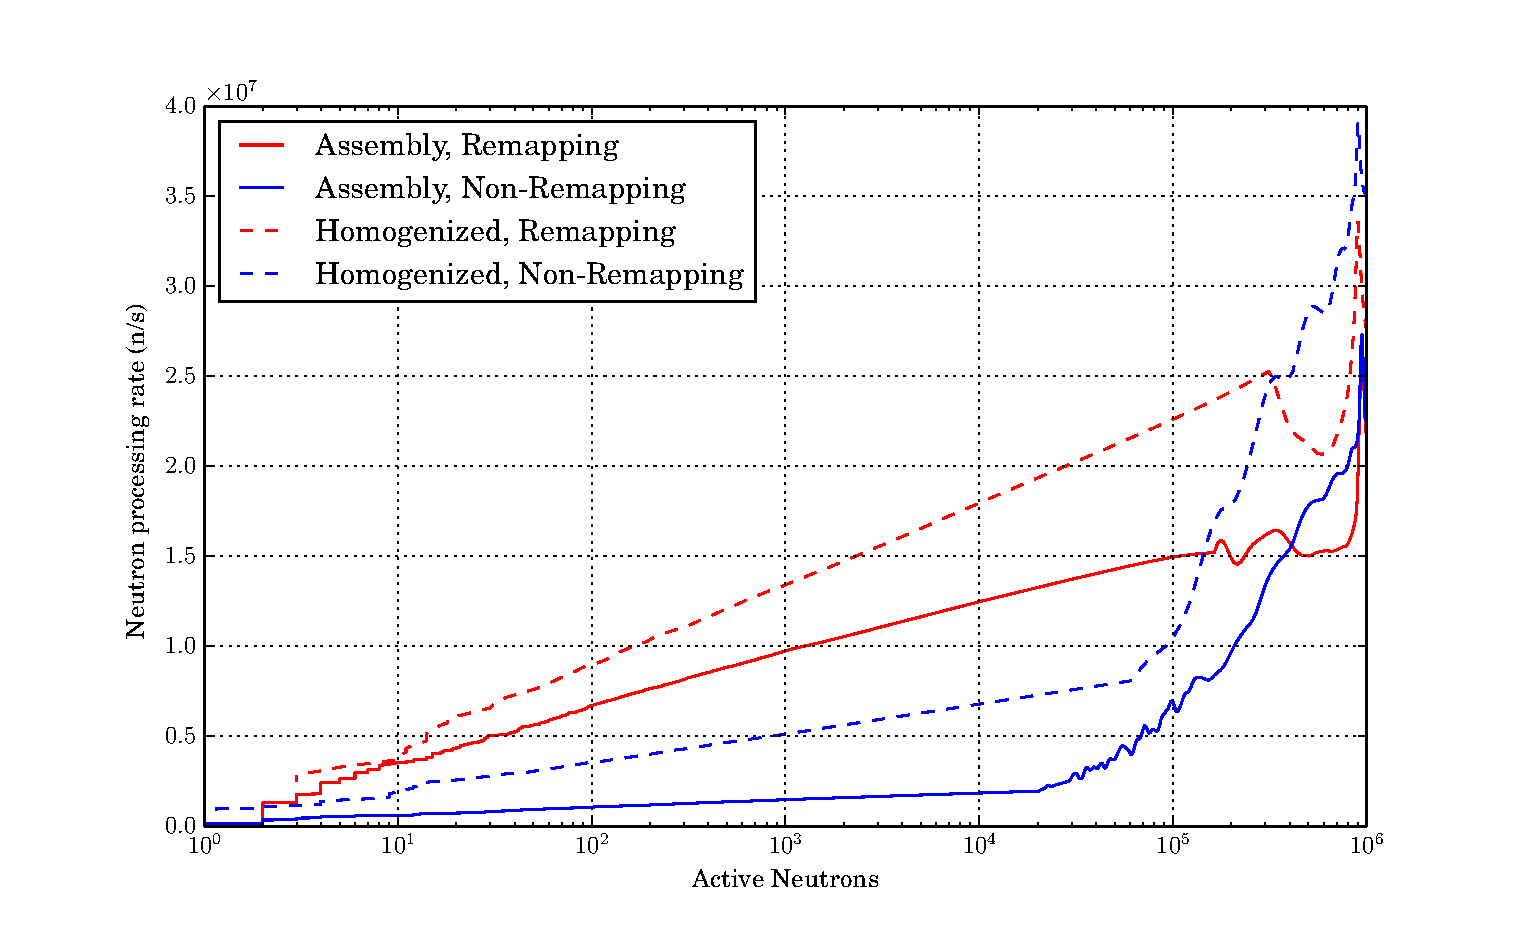
\includegraphics[width=\textwidth]{graphics/finalresults/process_rate.eps}
\caption{Neutron processing rate of WARP in the homogenized block and assembly benchmark cases. \label{process_rate} }
\end{figure}

\begin{table}[h!]
\centering
\caption{Summary table of the time spent in each WARP subroutine in criticality mode for each benchmark case.}
\label{profile_summary}
\begin{tabular}{| l | r  | r | r | r |}
\multicolumn{5}{l}{Remapping} \\
 \hline
 Subroutine        & Jezebel & Homogenized Block & Pincell & 15-sided Hex Assembly  \\
 \hline \hline
 OptiX Trace       & 3.8       &    18.5                        &   26.5    &      41.1    \\ \hline
 Grid Search       & 0.5       &    6.5                         &   5.1       &      4.7       \\ \hline
 Tally                   & 0.2       &    1.3                         &   0.5       &      0.4       \\ \hline
 Macroscopic      & 1.7       &   22.3                        &   19.2      &     19.0     \\ \hline
 Microscopic       & 1.3       &    11.3                        &  8.6        &      8.4       \\ \hline
 Radix Sort         & 1.7       &     5.3                         &   8.5       &      10.3     \\ \hline
 Elastic Scatter   & 1.0       &     15.1                       &   14.6    &      11.1    \\ \hline
 Inelastic Scatter & 0.4       &     0.4                         &   0.0      &       0.1   \\ \hline
 Continuum Scatter & 0.3   &     0.2                         &   0.0      &       0.1   \\ \hline
 Fission               & 0.2       &      0.2                        &   0.2      &       0.2     \\ \hline
 Yield Reduction  & 0.1       &      0.0                        &   0.0     &       0.0    \\ \hline
 Yield Rebase     & 0.0        &     0.0                         &   0.0     &       0.0   \\ \hline
 Yield Prefix Sum &  0.0       &    0.0                         &   0.0     &       0.0   \\ \hline
 Pop Source         &  87.3     &    18.3                       &   14.5   &      5.2    \\ 
\hline
\multicolumn{5}{l}{} \\
\multicolumn{5}{l}{Non-Remapping} \\
 \hline
Subroutine         & Jezebel & Homogenized Block & Pincell & 15-sided Hex Assembly  \\
\hline \hline
 OptiX Trace       & 14.2       &      38.0            &   46.7    &    45.2     \\ \hline
 Grid Search       &  1.3      &        6.3                 &  4.7     &     2.1      \\ \hline
 Tally                   &  0.2      &         0.7               &   0.4    &    1.2       \\ \hline
 Macroscopic      &  1.3     &          8.8               &  6.6      &    2.8     \\ \hline
 Microscopic       &  1.5      &          5.6               &  2.6     &    1.9       \\ \hline
 Elastic Scatter   &  2.5      &        10.5                 &   8.3    &   3.6      \\ \hline
 Inelastic Scatter & 1.2       &        1.6                  &  1.5    &    2.4    \\ \hline
 Continuum Scatter & 1.1  &         1.5                 &   1.6   &    2.4   \\ \hline
 Fission               &  0.4      &         0.7                 &   0.9   &    1.3      \\ \hline
 Absorption          & 0.3       &         0.6                 &   0.8   &    1.3      \\ \hline
Active Reduction  &  3.8      &        7.3                  &   11.2   &  20.1        \\ \hline
 Yield Reduction  &   3.4     &        6.2                 &  9.6    &    17.3     \\ \hline
 Yield Rebase     &    0.0     &       0.0                   &   0.0  &    0.0    \\ \hline
 Yield Prefix Sum &   3.3    &       6.1                    &  9.6   &    17.2    \\ \hline
 Pop Source         &  67.9     &     12.8                    & 5.7    &    0.5    \\ 
\hline
\end{tabular}
\end{table}



These effects are more clearly seen in the trends of Figure \ref{process_rate}.  This figure shows the rate at which each version is able to process neutrons vs the number of active neutrons left in the batch.  The figure has been smoothed with a window 11 data points wide, and linearly interpolated where the timings were too close together and gave Inf or NaN results for processing rates.  The remapping version is slower at large numbers of active neutrons since accessing the entire dataset generally yields active data anyway.  Conversely, the remapping version is faster when there few active neutrons left in the batch and accessing the entire grid generally yields terminated data.  The tradeoff in the remapping version is that the sort adds overhead when there are many active particles, but eliminating completed data and thus reducing the grid size makes it much more efficient when there are few active neutrons left.  Since the radix sort is a very efficient operation, the addition cost is small in the (about 30\% slower), but the benefit at small neutron numbers pays for this (about 3x faster).   In the non-remapping version, the addition cost at low numbers of active neutrons is due to launching a large grid where most of the blocks access terminated data and simply return without doing work.  Compute cycles and, more importantly, loads from global memory are wasted simply to check if a neutron is terminated already or not.

It therefore makes sense that the remapping version performs much better when the simulation spends significant time in the sub-300k active neutrons region on the processing rate curve (about where the lines cross).  In the Jezebel, homogenized block, pin cell, and assembly benchmarks, 90\%, 77\%, 91\%, and 96\% of the transport iterations occur in this region, respectively.  It also makes sense that the relative number of iterations  spent in the regions is vaguely constant.  The particles die out exponentially, and it takes roughly the same number of transport iterations to go from $10^7$ to $10^6$ active neutrons as it does to go from $10^2$ to $10^1$ active neutrons.  This is why Figure \ref{process_rate} is plotted logarithmically in $x$, to emphasize that equal spaces under the curves  typically take the same amount of iterations to complete.  This shouldn't be confused for the amount of time the iterations take to complete, however.  Iterations with more active neutrons typically take more time to complete, but have overall higher processing rates since the large neutron payload pays for overheads and latencies.

In a high leakage problem, like Jezebel, or a highly absorbing problem, like the homogenized block, the neutrons die off quickly.  This means that the simulation is generally on a higher processing rate than problems where neutrons do not die off fast.  This is because the active neutrons population ``leaps'' down the curve faster and can skip very slow processing regions, especially at the end of the simulation where 10 particles can suddenly become 0, effectively skipping a large portion of slow processing.  Adding many surfaces also keeps neutrons alive longer, since they often have to resample the materials as they cross boundaries.  

Table \ref{profile_summary} shows a breakdown of the amount of time spent in each subroutine in the remapping and non-remapping versions of WARP.  The values shown are average values for an entire simulation.  The values will also will not add to 100\% since there are many other kernels launched and memory copies made, but these are typically only done at problem startup and are negligible compared to those listed.  The kernels included in the table are the compute kernels of the inner and outer transport loops.  

In the non-remapping version, WARP spends most of its time in global routines like OptiX, macroscopic, scan, and source pop kernels, whereas the remapping version spends most of its time in OptiX and the reaction kernels (except in the Jezebel benchmark, where almost all time is spent in the source pop).  This is due to the fact that the non-remapping version never knows where the active data is and must launch kernels over the entire grid at every iteration.  This makes the global operations expensive since they are always going through $10^6$ elements.  In the remapping version, the global functions access the remapping vector and only sort or scan the active data, making them much cheaper as neutrons are terminated.  Remapping is almost always worth the effort, especially since radix is done in-place rather than having to be done and copied, but its main benefit is by eliminating stale access, and therefore grid size, not reducing divergence in the reaction kernels.

In its current state, the source pop operation is rather expensive, usually in the top five most costly routines.  This may explain why the fixed source mode is much slower that the criticality mode.  In fixed source mode, the source pop needs to be done at every inner loop iteration to add active particles to the list of  active neutrons, whereas in criticality mode it is only done once at the end of the inner loop.



